\documentclass[a4paper, 10pt]{article}
\usepackage{pgf}
\usepackage{eurosym}
\usepackage{graphicx}
\usepackage{wasysym}
\usepackage{hyperref}
\usepackage{listings}
\usepackage{pxfonts}
\usepackage{verbatim}
\usepackage{color}
\usepackage{xcolor}
\usepackage{wrapfig}
\usepackage{enumitem}
\usepackage{booktabs}
\usepackage{tabularx}

\hypersetup{
    bookmarks=true,         % show bookmarks bar?
    unicode=true,          % non-Latin characters in Acrobat’s bookmarks
    pdftoolbar=true,        % show Acrobat’s toolbar?
    pdfmenubar=true,        % show Acrobat’s menu?
    pdffitwindow=true,     % window fit to page when opened
    pdftitle={Assignment 2},    % title
    pdfauthor={Paul Vesey},     % author
    pdfsubject={Construction Project Management},   % subject of the document
    pdfcreator={},   % creator of the document
    pdfproducer={xelatex}, % producer of the document
    pdfkeywords={'Project Management' }, % list of keywords
    pdfnewwindow=true,      % links in new PDF window
    colorlinks=true,       % false: boxed links; true: colored links
    linkcolor=violet,          % color of internal links (change box color with linkbordercolor)
    citecolor=magenta,        % color of links to bibliography
    filecolor=red,      % color of file links
    urlcolor=blue           % color of external links
}

\setlength\parindent{0pt}
\begin{document}

\lstset{language=HTML,
				basicstyle=\small,
				breaklines=true,
        numbers=left,
        numberstyle=\tiny,
        showstringspaces=false,
        aboveskip=-20pt,
        frame=leftline
        }
				
\begin{table}%
	\begin{minipage}{0.4\textwidth}%
			
\includegraphics[width=1\textwidth]{./img/LITlogo.jpg}
	\end{minipage}
	\qquad
	\centering
	\parbox{0.4\textwidth}{
		\begin{large}			
			\begin{tabular}{| r | l |} \hline
				Subject: & \textbf{Construction Project Management}\\
				Course: & \textbf{CPM Special Purpose Award}\\	
				Session: & \textbf{Spring 2020}\\
				Lecturer: & \textbf{Paul Vesey \footnotesize{BEng, MIE, HDip}}\\
				\hline
			\end{tabular}
		\end{large}			
	}
\end{table}
\vspace{0.25cm}	

%     _            _                                  _     _  _   
%    / \   ___ ___(_) __ _ _ __  _ __ ___   ___ _ __ | |_  | || |  
%   / _ \ / __/ __| |/ _` | '_ \| '_ ` _ \ / _ \ '_ \| __| | || |_ 
%  / ___ \\__ \__ \ | (_| | | | | | | | | |  __/ | | | |_  |__   _|
% /_/   \_\___/___/_|\__, |_| |_|_| |_| |_|\___|_| |_|\__|    |_|  
%                    |___/                                         

\begin{flushleft}
\Large\textbf{Practical 4 - Baselines, Graphics Panel}\\
\end{flushleft}

In this exercise we are going to explore some key functionality available in MS Project.  Specifically, we are going to examine:

\begin{enumerate}
	\item Baselines
	\item Slippage / Slack
\end{enumerate}

You have been provided with a simple .mpp file to get you started.  This is available on Moodle.\\
Following a demonstration, you are required to:

\begin{enumerate}
	\item Set a Baseline - 'Baseline'
	\item Show the 'Actual Start' column
	\item Set the Actual Start of Task A and Task B to be two days after the original planned starts.
	\item View Impact of this change on the graphics panel
\end{enumerate}

To view various aspects of the impact you will need to right-click on the graphics panel and switch on Baselines, Critical Task, Slippage, etc.\\

Next you will need to create another baseline, which in this case we are going to use to record the impact of a change in scope.  For the purpose of this assignment we are going to increase the duration of Task R and then Task S.  In each case we are going to increase the durations by 2 days.

\begin{enumerate}
	\item Set Baseline 1
	\item Show Baseline 1 Duration column
	\item Increase the duration for Task R by two days
	\item Observe and record the impact
	\item Increase the duration for Task S by two days
	\item Observe and record the impact
\end{enumerate}


\begin{figure}[hb]
	\centering
		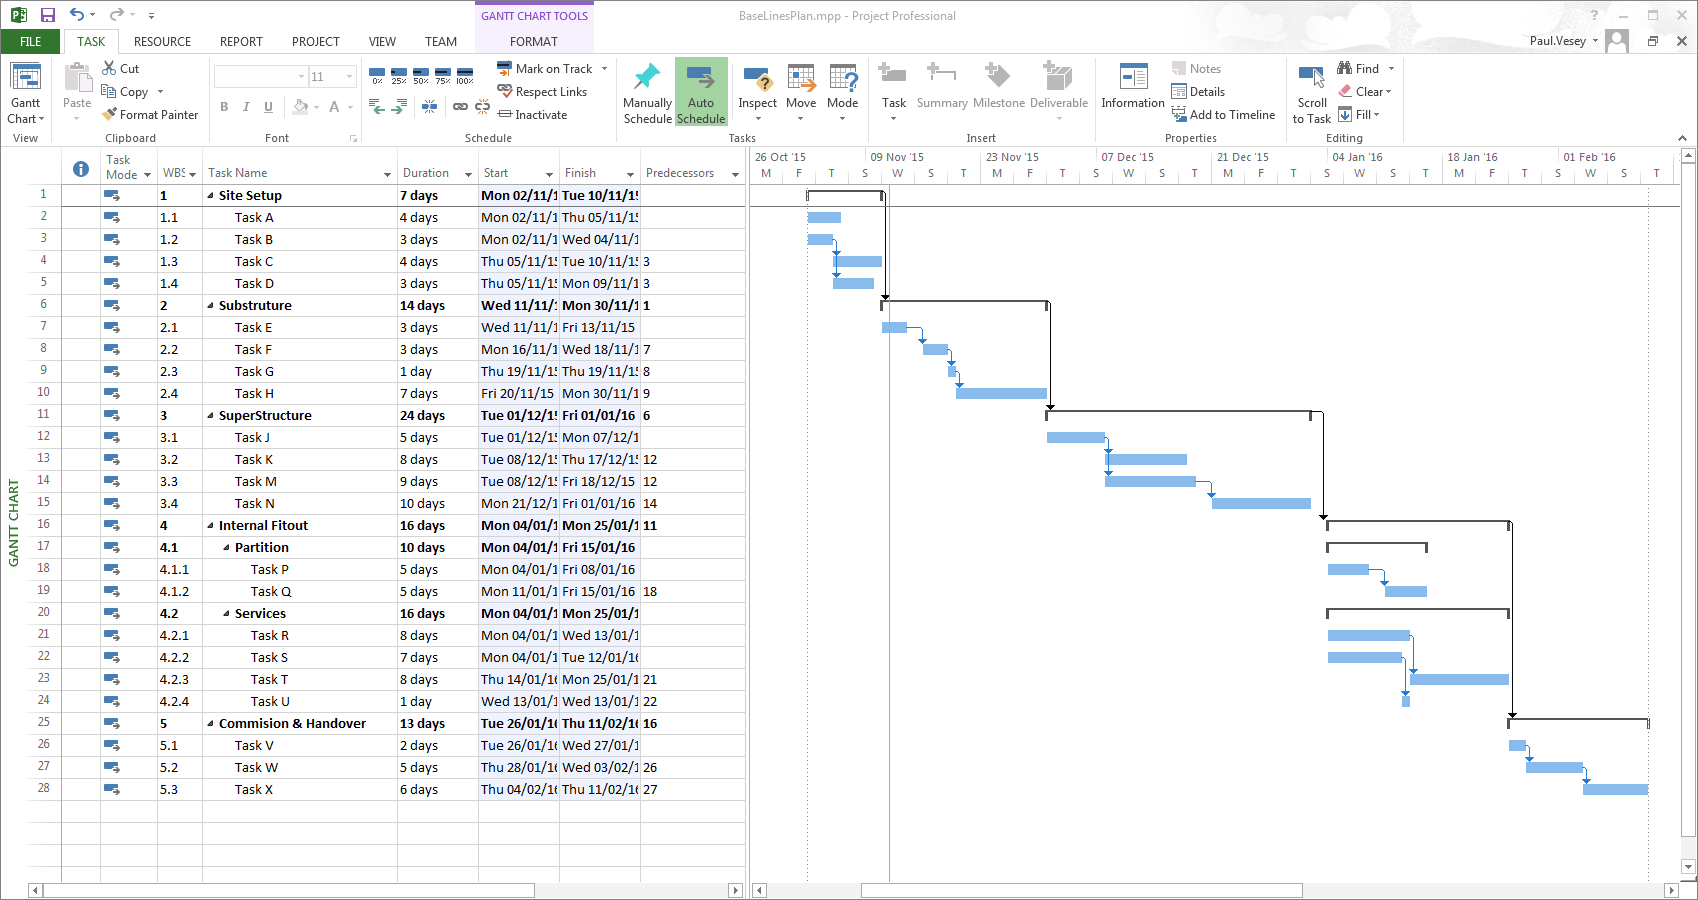
\includegraphics[width=1.00\textwidth]{img/P4ProjectPlan.PNG}
	\caption{Exercise Start Point}
	\label{fig:P4ProjectPlan}
\end{figure}


\begin{figure}[hb]
	\centering
		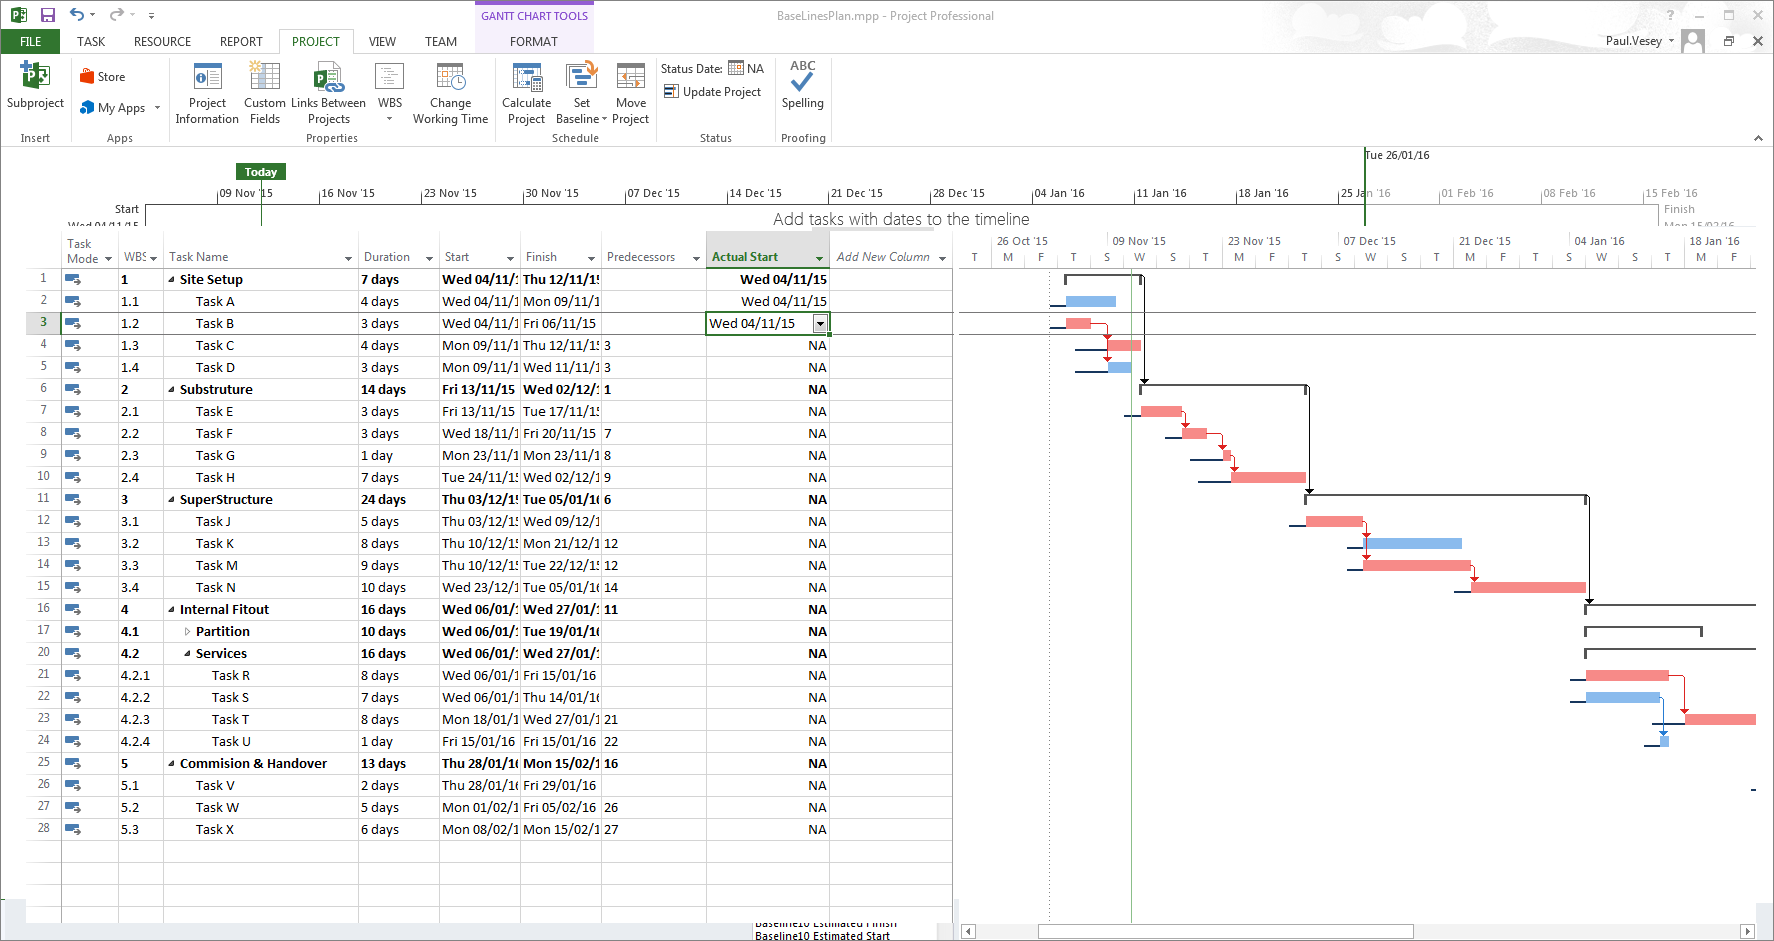
\includegraphics[width=1.00\textwidth]{img/CriticalTasks.PNG}
	\caption{Critical Tasks On}
	\label{fig:P4Critical}
\end{figure}



\begin{figure}[hb]
	\centering
		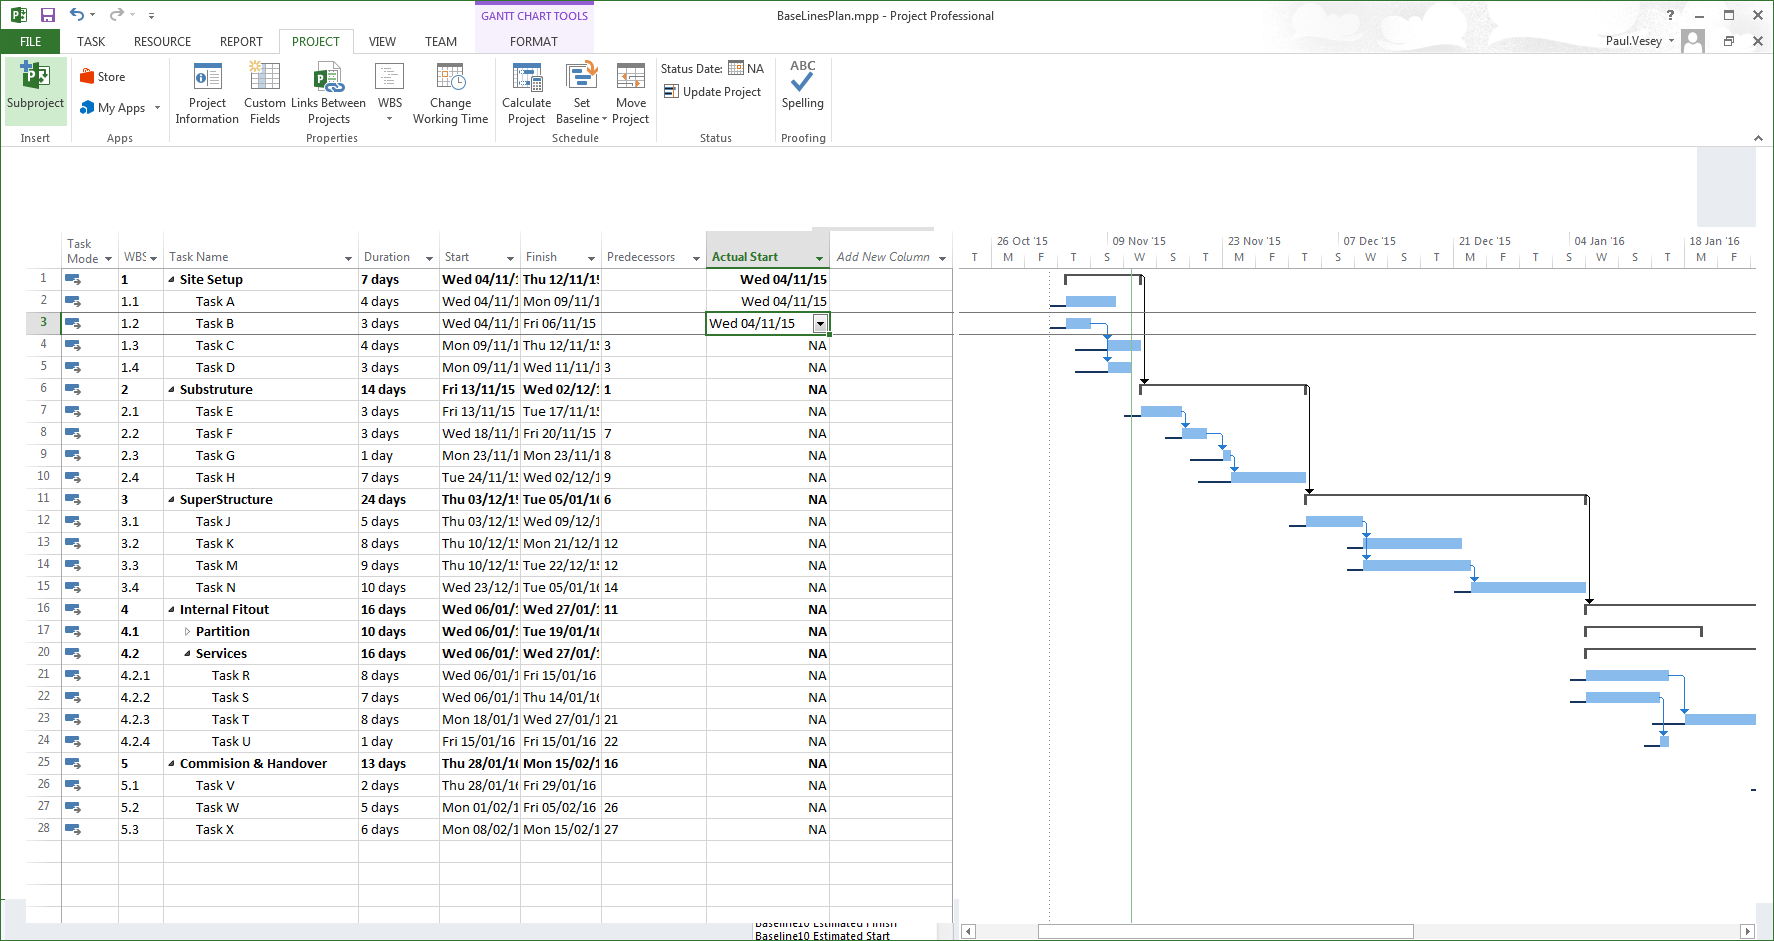
\includegraphics[width=1.00\textwidth]{img/Slippage.PNG}
	\caption{Slippage turned On}
	\label{fig:P4Slippage}
\end{figure}

\begin{figure}[hb]
	\centering
		\includegraphics[width=1.00\textwidth]{img/Baselines.PNG}
	\caption{Baselines Shown}
	\label{fig:P4Baseline}
\end{figure}

\end{document}